\begin{figure}[p]
\centering
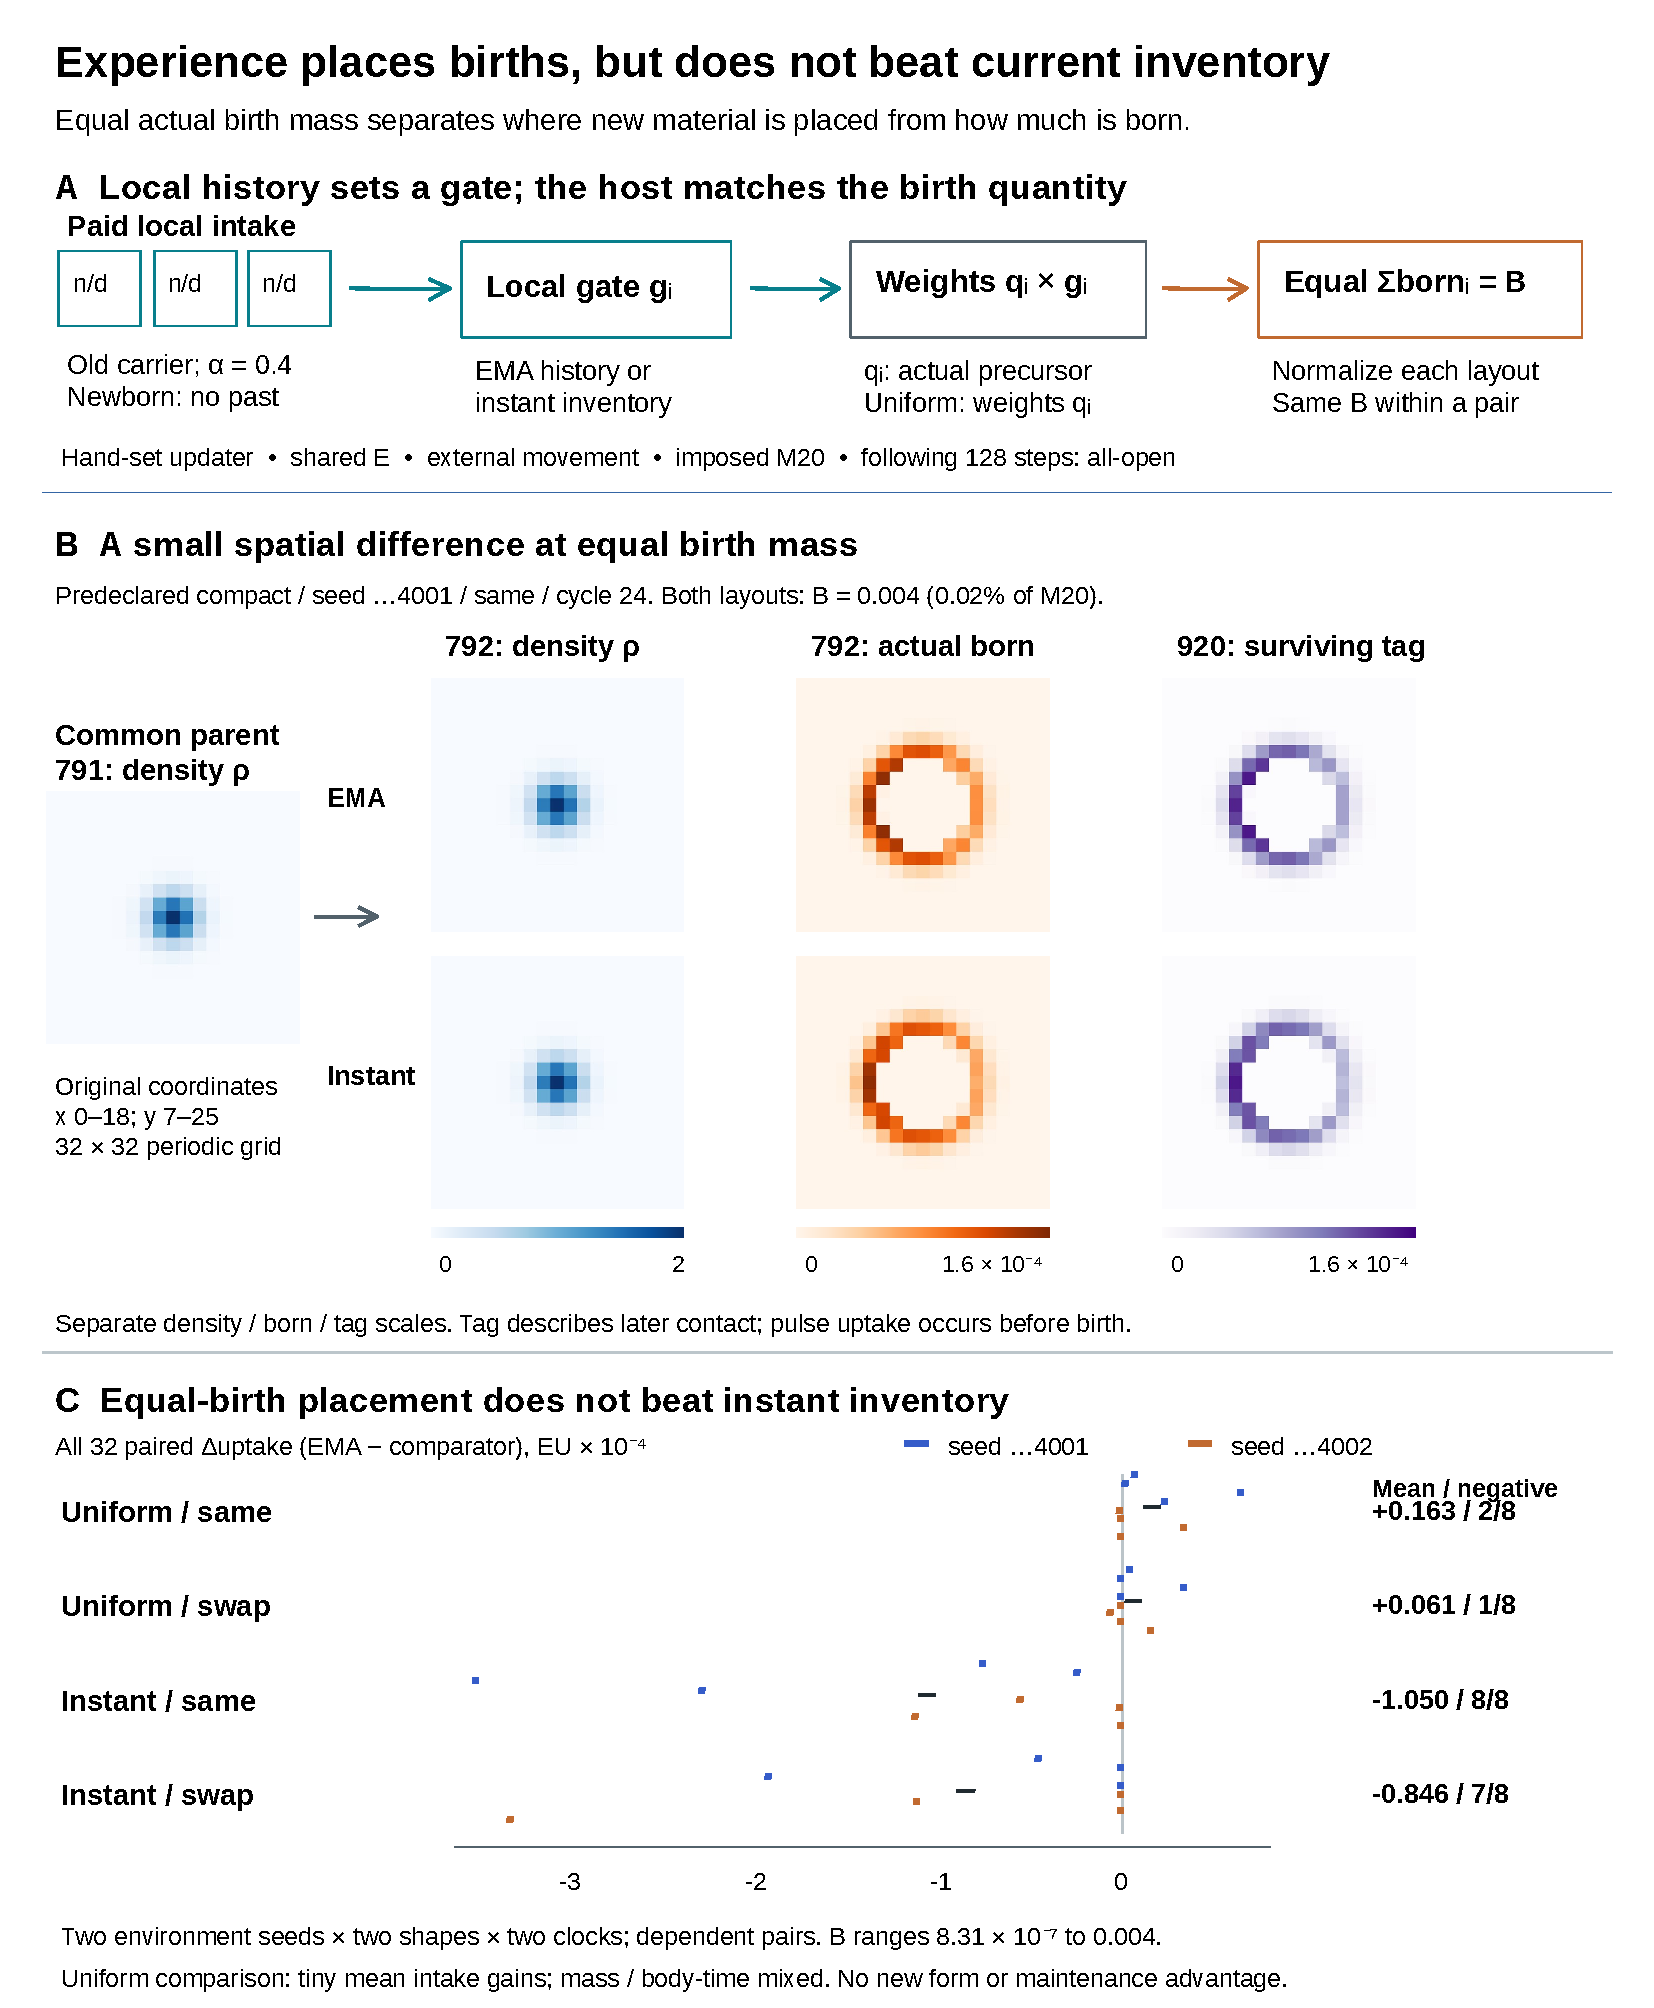
\includegraphics[width=\linewidth,height=0.77\textheight,keepaspectratio]{work/method_renewal/figures/birth_placement/birth_placement.pdf}
\captionsetup{font=footnotesize}
\caption{\textbf{History changes material placement but does not outperform current inventory in matched small births.}
\textbf{A,} Completed local intake supplies a hand-set, material-carried EMA and a birth gate. The host matches total admitted mass $B$ within each history/uniform or history/instantaneous-resource pair; the policy does not observe its returned precursor $q$. Movement, shared energy and the mass cap remain prescribed.
\textbf{B,} Predeclared compact body, seed 202610184001, unchanged ports: saved parent 791, birth 792 and tag 920. Crop fixed in original coordinates; density and material scales differ. Both arms admit $B=0.004$, 0.02\% of the mass cap. Tags start after pulse uptake. For fully paid, nonreproducing tags, uniform turnover fixes total retention, not contact. Tags do not measure energy flow. Recovery shares a requested movement tape and 128 all-open steps.
\textbf{C,} All 32 paired differences in subsequent whole-body uptake, in the displayed $10^{-4}$ units. Colours identify the two environmental seeds; black marks are arithmetic means, not uncertainty intervals. Shapes, pulse times and futures are dependent. History gains slightly over uniform gating of actual precursors, but loses to current inventory in 15 of 16 pairs; mass and body-time effects do not uniformly follow uptake. The intervention does not establish a new morphology or a learned update rule.}
\label{fig:birth-placement}
\end{figure}
